\documentclass[border=6pt]{standalone}
\usepackage[T1]{fontenc}\usepackage{lmodern}\usepackage{amsmath,amssymb}\usepackage{graphicx}\usepackage{xcolor}\usepackage{tikz}
\usetikzlibrary{arrows.meta,positioning,calc,fit,shapes.misc,shapes.geometric}
% TikZ styles
\tikzset{
  blk/.style={draw, rounded corners=2pt, align=center, font=\small, minimum height=8mm, inner sep=4pt, fill=#1},
  blk/.default=white,
  arr/.style={-{Stealth[length=2.2mm]}, thick},
}
\definecolor{base}{HTML}{FBE3E3}
\definecolor{prop}{HTML}{DDEBFA}
\definecolor{same}{HTML}{EDEDED}
\definecolor{done}{HTML}{DFF1DF}
\definecolor{todo}{HTML}{FFF2CC}

\begin{document}
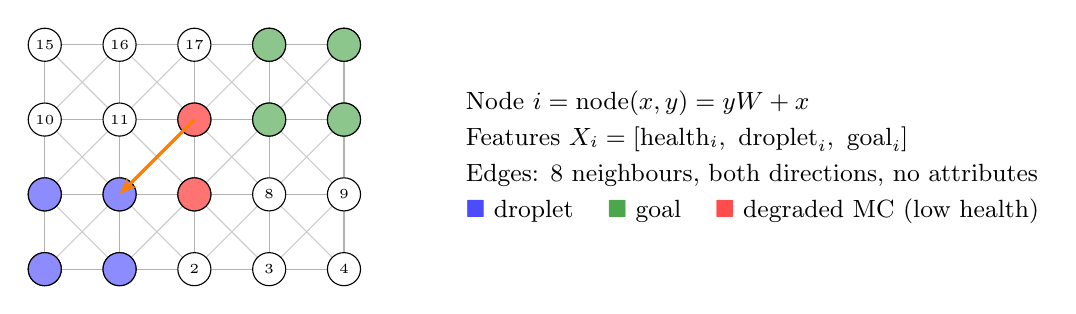
\begin{tikzpicture}[scale=0.95]
  \foreach \x in {0,...,4} \foreach \y in {0,...,3} {
    \ifnum\x<4 \draw[gray!60] (\x,\y) -- (\x+1,\y); \fi
    \ifnum\y<3 \draw[gray!60] (\x,\y) -- (\x,\y+1); \fi
    \ifnum\x<4 \ifnum\y<3 \draw[gray!40] (\x,\y) -- (\x+1,\y+1); \draw[gray!40] (\x+1,\y) -- (\x,\y+1); \fi\fi }
  \foreach \x in {0,...,4} \foreach \y in {0,...,3}
    \node[circle, draw, fill=white, inner sep=0pt, minimum size=4.2mm, font=\tiny] at (\x,\y) {\pgfmathparse{int(\y*5+\x)}\pgfmathresult};
  \foreach \p in {(0,0),(1,0),(0,1),(1,1)} \node[circle, draw, fill=blue!45, inner sep=0pt, minimum size=4.2mm] at \p {};
  \foreach \p in {(3,2),(4,2),(3,3),(4,3)} \node[circle, draw, fill=green!50!black!45, inner sep=0pt, minimum size=4.2mm] at \p {};
  \foreach \p in {(2,1),(2,2)} \node[circle, draw, fill=red!55, inner sep=0pt, minimum size=4.2mm] at \p {};
  \draw[arr, orange, very thick] (2,2) -- (1,1);
  \node[align=left, font=\small, anchor=west] at (5.5,1.5)
    {Node $i=\mathrm{node}(x,y)=yW+x$\\[2pt]
     Features $X_i=[\text{health}_i,\ \text{droplet}_i,\ \text{goal}_i]$\\[2pt]
     Edges: 8 neighbours, both directions, no attributes\\[2pt]
     \textcolor{blue!70}{$\blacksquare$} droplet \quad
     \textcolor{green!50!black!70}{$\blacksquare$} goal \quad
     \textcolor{red!70}{$\blacksquare$} degraded MC (low health)};
\end{tikzpicture}
\end{document}
